\input{chapter-header.tex}
% ===========================================================================
\chapter{The \Vtt Prototype}
\minitoc
\chaplabel{prototype}
% ===========================================================================
\introduction
% ===========================================================================

To validate our model, we implemented our \Vtt prototype on the Pharo platform~(Section \ref{sec:pharo_execution_model}). Our solution virtualizes Pharo application runtimes and provides, as already described, the ability to manipulate their object graph and control their execution. Our implementation includes a language side library containing the object space and language hypervisor related classes. Our main modification to Pharo is an extension to its stack-based \VM. This \VM is a version of the Pharo \VM without a Just In Time~(JIT) compiler. Our extension allows the co-existence of several application runtimes on the same \VM and the modification of the \VM setup interface.

An object space VM-Setup Interface in \Vtt is implemented by exposing Pharo's \emph{special objects array}~(Section \ref{sec:setup_interface}). The \emph{special objects array} is an array which contains references to the objects that the \VM may need at runtime. The special objects is used by the Pharo \VM with two main purposes. On one side it serves as a container for the \VM setup configuration by referencing all the special objects the interpreter may need at runtime. On the other side it provides an entry point holding the \VM interpreter state \ie we could reuse the same interpreter with several purposes by replacing its special objects array. This last feature provides support for the execution of several application runtimes on top of the same \VM. In our solution, the \VM has a single bytecode interpreter shared amongst the different running runtimes. To allow the execution of a different runtime, we exchange the interpreter state~(the special objects array) by the state of its corresponding runtime in an atomic operation that we call \emph{context switch}~(Section \ref{sec:context_switch}).

\Vtt mirror implementation~(Section \ref{sec:implementation_mirrors}) does not require particular changes in the Pharo \VM. We base our mirror implementation in two existing \VM primitive operations that allows us to execute a primitive on an arbitrary object by changing the primitive's receiver. Additionally, the already existing reifications of objects such as \ct{CompiledMethod}, \ct{Process}~(threads) and \ct{Context}~(stack frames or activation records), allow us to manage such runtime elements using the same mirror mechanism and avoid the development of specific ad-hoc solutions.

\Vtt's presents a memory layout where the objects of both the virtualized and hypervisor co-exist in the same heap~(Section \ref{sec:memory}). This means that there is no need for special support on \emph{cross-runtime references} for implementing \eg mirrors, and that we can reuse the existing memory management in the virtual machine almost transparently.
However, this solution forbids us to analyze the memory usage of the virtualized runtime and has an impact on the GC.

This chapter finishes, with means of completion, by presenting the non-implemented aspects of our solution: JIT compilation, shared state enforced by \VM implementation and correct management of external resources such as files or sockets~(Section \ref{sec:not_yet_implemented}).

\section{Pharo Execution Model in a Nutshell}\label{sec:pharo_execution_model}

To understand the constraints and limitations of our solution, we start this chapter by presenting the execution model imposed by the Pharo \VM. The Pharo \VM features a bytecode-based stack interpreter with a generational garbage collector and a JIT compiler. For the interested reader, several publications describe its details and how it evolved during time~\cite{Gold83a,Inga97a,Mira11a}. On the execution model side, this \VM imposes us the following contract:

\begin{description}

\item[Object Format.] All objects in the 32 bit version of the Pharo \VM have a header and a list of fields. The object header is one, two or three words long and describes amongst others how large is the field list of the object, if those fields contain weak or strong pointers, and which is the class of the object. The \VM also assumes the format of other special objects such as classes, method dictionaries and methods. Each class must have three mandatory fields: the class' superclass, a method dictionary used during the method lookup and an integer describing the class format. Method dictionaries are hash tables using as hash function the identity of the object. Methods are objects that contain a list of bytes with the bytecodes of the method and a list of the literal objects of that method encoded in the bytes.

\item[Object Model.] The Pharo \VM enforces, in its lowest level, a class-based object oriented model with single inheritance. Each object has a reference to its class~(that appears inside its header). Each class has only one superclass~(or \ct{nil} denoting the end of the hierarchy) and one method dictionary. The \VM during its execution does not enforce the existence of metaclasses nor a particular class hierarchy. Instead, meta-classes are build on top of this much simpler model. Indeed, this simple model allows one to implement other language extensions such as Traits~\cite{Scha03a} or the decomposition of the language reflective behavior such as in Metatalk\cite{Papo11a}.

\item[Bytecode set.] The Pharo \VM constrains methods to a limited amount of predefined bytecode sets. These bytecode sets are based on the \VM's stack based interpreter. This means that every language that is meant to run on top of this \VM must be compiled to any of these bytecode sets, independently of its original syntax and semantics. 

\end{description}

\section{The Special Objects Array as \VM-Setup Interface}\label{sec:setup_interface}

Pharo \VM holds the state of the \VM-setup interface inside a \emph{special objects array} object. Pharo's special objects array contains 56 entries whose indexes are well known by the \VM for their access at runtime. To implement our \VM-setup interface, we expose, access and modify this special object array. Following, we detail the special objects array entries that we expose for our solution.

\begin{description}
\item[Special Instances.] Special instances such as \ct{nil}, \ct{true} and \ct{false} are directly pushed by the \VM interpreter at runtime instead of residing in a method literal list. A flyweight \ct{Character} table contains the first 256 character objects to ensure their identity and save memory.

\item[System Dictionary.] The system dictionary contains all installed classes in the system. An object space uses this entry to query the installed classes and to install new ones. The \VM does not make any special use of this object as it is managed directly from the language.

\item[Process Scheduler.] The process scheduler contains all existing processes/threads in the runtime. We can install and remove process from the process scheduler. The \VM uses this same process scheduler to manage the runtime's execution.

\item[Symbol Table.] The symbol table gathers is the set of \emph{unique} strings in the system. Symbols are mainly used to denote method signatures and ensure reference equality during the method lookup. An object space uses the symbol table to map symbols between runtimes and so it ensures no duplicate symbols are created. The \VM does not make any special use of this object as it is managed directly from the language.

\item[Literal Classes.] Literal classes are the classes of literal objects. Literal objects are those present directly in a method's literal list~(\eg numbers, strings, literal arrays), or those objects that the \VM creates at runtime~(\eg BlockClosures). On one side, the \VM uses the classes available in this list to directly instantiate objects of these types or perform safety checks at runtime~(which cannot be performed at compile time because of reflection or the dynamically-typed nature of the language). On the other side, an object space uses these well-known classes to perform transformations between objects in one runtime to another \eg translate a string from the hypervisor runtime to a string in the virtualized runtime.

\item[Special Selectors.] The special selectors denote those messages that the \VM will send to the image under special situations. This is the case of the \ct{doesNotUnderstand} selector that is sent to the receiver object when the method lookup fails finding a method under a message-send. Other selectors in this category are (a) \ct{cannotInterpret} which is sent when a class in the middle of the method lookup has no method dictionary, (b) \ct{mustBeBoolean} which is sent when a branch operation founds a non-boolean object, (c) \ct{cannotReturn} and \ct{aboutToReturn} are selectors used when stack frames are finalized or being finalized respectively and (d) \ct{run:with:in:} is the message used to implement method wrappers.

\end{description}



%Particularly, the special objects array contains a process scheduler object and its corresponding process objects, implementing green threads. Pharo virtual machine has a single threaded nature and uses green threads to organize its execution.

\section{Cycle Execution and Context Switch} \label{sec:context_switch}

The Pharo \VM has single threaded execution. Only one operating system thread is used to execute Pharo code, so process scheduling is handled internally by the virtual machine. Processes scheduled using this approach are also called \emph{green threads}. Green threads provide process scheduling without native operative system support while limiting the proper usage of modern multicore CPUs. By using green threads only one process, the \emph{active process}, is executed at each instant in time. After the active process executes for a given window of time, if there are any waiting processes with greater or equal priority, the active process gets preempted \ie it is suspended and the process with the highest priority becomes the new active process.

In \Vtt, we modified part of the green thread mechanism to allow the scheduling of different language runtimes. We call \emph{context switch} the mechanism that changes from one language runtime to another. A virtualized language runtime runs for a window of time after which it gets preempted if another runtime with highest priority~(the language hypervisor runtime) is waiting. Internally, the \VM has a single bytecode interpreter shared amongst the different running runtimes. To perform the context switch, we exchange the special objects array of the \VM interpreter by the one in the language runtime to resume, and then resume the \VM execution. This solution keeps the single threaded nature of the \VM meaning that when a language runtime is running the others are suspended. This implementation has the benefit of avoiding concurrency problems between the different language runtimes, allowing us to focus on the runtime modification features.


\begin{figure*}[htb]
\begin{center}
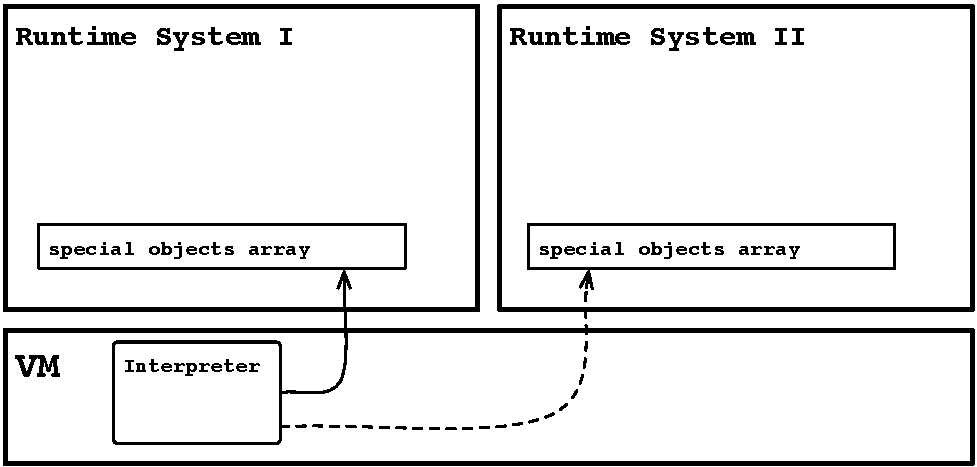
\includegraphics[width=.8\linewidth]{object_space_context_switch}
\caption{\textbf{Context Switch Internals.}To perform a context switch, we change the special objects array of the \VM's interpreter.\label{fig:context_switch}}
\end{center}
\end{figure*}

Finally, the window time control was implemented reusing the existing process preemption mechanism in the \VM. A separate thread, namely the \emph{heartbeat}, is awaken every 200 milliseconds and activating a flag that indicates a preemption may occur. When the \VM code interpreter arrives to one of the safe suspension points (\ie a point where suspending the current execution will not leave the current process in a incoherent state) the code interpreter preempts the active process if the corresponding flag was activated. Such safe suspension points are in our implementation the back jump and message-send bytecodes. These suspension points avoid to suspend the execution in between of \eg operations that perform stack alignment. In \Vtt we modified the preemption code to activate another language runtime if available.

\section{Mirror Implementation}\label{sec:implementation_mirrors}

Our mirror implementation manipulate the objects inside an object space by using already Pharo \VM primitives. A primitive in Pharo is a function executed at the \VM level. To execute a primitive from the language, this primitive should be available as a method. Then, we have to send the corresponding message to the object subject of the primitive:

\begin{code}
Array >> size [
    <primitive: 62>
]

{1 . 2 . 3} size.
\end{code}

We want however, to avoid cross-runtime message-sends, we bypass the message-send with the combination of two existing primitives:
\begin{description}
	\item \textbf{Execute a given method on an object.} Given a method, it is possible to execute it on an object, avoiding method lookup in the object. In current Pharo \VM, this primitive is implemented in the method \textbf{\ct{receiver:withArguments:executeMethod:}} of the \ct{CompiledMethod} class, with number 188. This method receives as arguments the object on which the primitive will be executed, an array of arguments, and the methods to execute.
	\item \textbf{Execute a primitive on an object.} It is possible to send a message to an object, so a primitive is executed on the receiver. This primitive is implemented in Pharo's \ct{ProtoObject} class as \textbf{\ct{tryPrimitive:withArgs:}} with number 118 and receives as argument the number of the primitive and an array or arguments.
\end{description}

We use primitive \ct{receiver:withArguments:executeMethod:} to execute the primitive method \ct{tryPrimitive:withArgs:} on the object from the virtualized runtime, avoiding the \emph{cross image-message send} and executing directly the primitive on the given object.

\begin{code}
CompiledMethod
       receiver: anObjectFromOtherRuntime
       withArguments: { aPrimitiveNumber . anArrayOfArguments }
       executeMethod: (ProtoObject >> #tryPrimitive:withArgs:)
\end{code}

Our \Vtt prototype includes one mirror per type of object supported by the Pharo \VM. Notice that as some runtime elements such as methods, activation records or even processes are reified as objects in Pharo, we can manipulate them through mirrors without developing new support for them in the \VM:

\begin{description}
\item[Object mirrors.] Mirrors for objects containing just object references such as an \ct{Array} or an \ct{OrderedCollection}.
\item[Word mirrors.] Mirrors for objects containing only non-reference word fields such as a \ct{Float} or a \ct{WordArray} object.
\item[Byte mirrors.] Mirrors for objects containing non-reference byte size fields such as a \ct{ByteArray} or a \ct{ByteString}. 
\item[Class mirror.] Mirrors for class like objects. They control the manipulation of classes and honor the format of a class in the Pharo \VM which should necessary have as its first three instance variables the superclass of the class, its format and method dictionary.
\item[Method dictionary mirror.] Mirrors for method dictionaries honoring the \VM invariants for method installation \ie using the identity hash of the key object instead for doing the lookup in the method dictionary.
\item[Method mirror.] Mirrors for method objects. Method objects in the Pharo \VM are objects with a mixed format. They contain object references to their literals, and byte fields with their bytecode.
\item[Context mirror.] Mirror for context objects. A context object is reified lazily by the Pharo \VM and contains a variable amount of fields denoting the local variables of a scope.
\item[Process mirror.] Mirror for process objects. Process objects are used to manage the execution of a Pharo runtime. They can be resumed, suspended or finalized.
\end{description}


%Using Oz, we can also create and install new processes inside an \objectspace given a code expression. The creation of a process requires the creation of a compiled method with the code~(bytecode) corresponding to the desired expression and a method context. The compiled method with the code to run is obtained by compiling the expression in the host and creating an \objectspace compiled method. The \objectspace compiled method is then provided with the compiled bytecode and its corresponding literals.

\section{Memory Layout} \label{sec:memory}

In \Vtt, all objects belonging to the different language runtimes share a unique object heap. Objects are mixed in this heap and are objects from the same language runtime not necessarily contiguous, as shown in Figure \ref{fig:heap}. However, Although they are mixed, they are logically separated as they conform different object graphs. Pharo being a safe-language~\cite{Hawb98a,Hawb02a} prevents us to forge references~(\ie creating references from numbers using pointer arithmetic) and isolates the object graphs of each runtime system.

\begin{figure}[ht]
\begin{center}
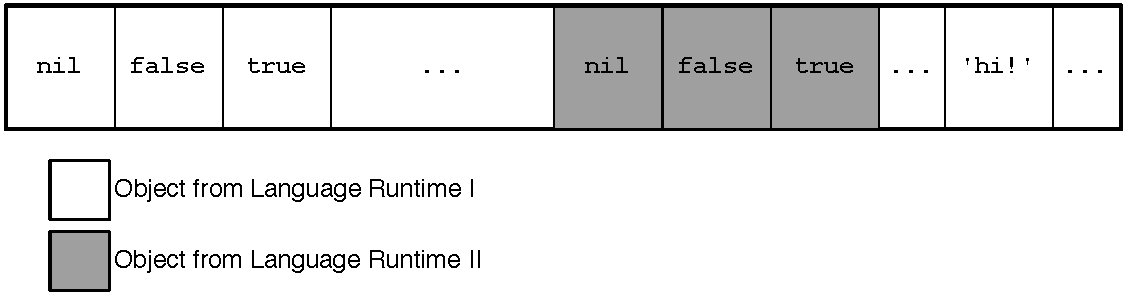
\includegraphics[width=.9\linewidth]{object_spaces_heap}
\caption{\textbf{A unique heap containing objects from different language runtimes.} Objects from the language runtime I and language runtime II are mixed in the heap. In this figure, after the \ct{nil}, \ct{true} and \ct{false} instances that belong to language runtime I, follow the corresponding ones of the language runtime II, which can in order be followed by objects of the former, like the string \textbf{`hi'}. \label{fig:heap}}
\end{center}
\end{figure}

This decision is funded on minimizing the changes made to the virtual machine, to minimize the complexity in our prototype implementation. Our decision, while easing the development of our solution, has the following impact on it:

\begin{description}
	\item[Reuse memory handling mechanisms.] We use the same existing memory infrastructure as when \Vtt is not used. Existing mechanisms for allocating objects or growing the object memory when a limit is reached can be reused transparently by our implementation. 
	\item[Simplify the object reference mechanism.] Cross-runtime references are normal object references. No extra support from the virtual machine was developed in this regard.
	\item[Shared garbage collection.] Since objects from the different runtimes are mixed in the object memory, and their boundaries are not clear from the memory point of view, the garbage collector~(GC) is shared between them. Every GC run must iterate over all their objects, increasing its time to run.
\end{description}

%This solution seems suitable  J-Kernel \cite{Hawb98a} and Luna \cite{Hawb02a} present a solution similar to ours regarding the memory usage. They are Java solution for isolating object graphs with security purposes. In them, each object graph is called a \emph{protection domain}. All protection domains loaded in a system, and their objects, share the same memory space. 

%The J-Kernel enforces the separation between domains by using the Java type system, the inability of the Java language to forge object references, and by providing capability objects\cite{Levy84a,Mill03a,Spoo00a} enabling remote messaging and controlling the communication. This same separation in Luna \cite{Hawb02a} is achieved by the modification of the type system and the addition in the virtual machine of the \emph{remote reference} concept. In our solution, the separation is given by the same inability to forge object references and the membrane objects that control the communication.

%\section{Creating an \objectspace} \label{sec:object_space_creation}
%
%An \objectspace can be created either from scratch or by loading an existing image. Loading an existing image was implemented as a virtual machine primitive, because the image snapshot is actually a memory snapshot and therefore, easier to handle at VM level. This primitive, implemented with the code shown in Figure~\ref{code:import_image}, reads the snapshot file, puts all objects into the object memory, updates the object references to make them coherent and finally returns the special objects array of the loaded image.
%
%\begin{figure}[htb]
%\begin{code}
%\textbf{primitiveLoadImage}
%    | headerlength bytesRead newImageStart rootOffset oldBaseAddress dataSize rootOop fileObject |
%    
%    "get the reference to the file object"
%    fileObject := self stackValue: 0.
%
%    "Where will we put the new objects"
%    newImageStart := objectMemory startOfFreeSpace.
%
%    "read image header"
%    self readLongFrom: fileObject.
%    headerlength := self readLongFrom: fileObject.
%    dataSize := self readLongFrom: fileObject.
%    oldBaseAddress := self readLongFrom: fileObject.
%    rootOffset :=
%          (self readLongFrom: fileObject) - oldBaseAddress.
%    
%    "seek into the file the start of the objects"
%    self seek: headerlength onFile: fileObject.
%    
%    "grow the heap in the ammount of the image size"
%    objectMemory growObjectMemory: dataSize.
%    
%    "read the file into the free part of the memory"
%    bytesRead := self
%                    fromFile: fileObject
%                    Read: dataSize
%                    Into: newImageStart.
%
%    "tell the vm the free space is now after the loaded objects"
%    objectMemory advanceFreeSpace: dataSize.
%         
%    "update the pointers of the loaded objects"
%    self
%          updatePointersForObjectsPreviouslyIn: oldBaseAddress
%          from: newImageStart
%          until: newImageStart + dataSize.
%    
%    "return the special objects array"
%    rootOop := newImageStart + rootOffset.
%    self pop: 2 thenPush: rootOop.
%\end{code}
%\caption{Implementation of primitive \textbf{\ct{primitiveLoadImage}} that loads an image snapshot into the object memory written in Slang
%\label{code:import_image}}
%\end{figure}
%
%On the other side, creating an \objectspace from scratch can be implemented as a bootstrap of the system, following the process defined in \cite{Poli12a}. The \objectspace provides the \textbf{\ct{createObjectWithFormat:}} method to create an object respecting the given format but with an anonymous class, so we can consider it as a "classless" object. This method is used in the first stage of the bootstrap process, when no classes are available in the \objectspace image yet, to create the \ct{nil} instance~(cf. Figure~\ref{code:bootstrap_nil}) and the first classes~(cf. Figure~\ref{code:bootstrap_classes}). Later, when the classes are available, those objects are set their corresponding ones by using the \textbf{\ct{setClass:}} message.

\section{Benchmarks}

To verify the feasibility of this model, we built our \Vtt prototype in the Pharo language. Our prototype includes the \Vtt class libraries and modification f the JIT-less version of the Pharo \VM.
We benchmarked the virtualized execution of our prototype implementation using a subset of the computer language benchmarks game\footnote{\url{http://benchmarksgame.alioth.debian.org/}}.

We executed each of these benchmarks ten times in two different setups. Results are found in Table \ref{tb:benchmarks}. We first benchmarked the Vanilla JIT-less Pharo \VM without any of our changes, to make it a fair base of comparison with our JIT-less solution. Following, we benchmarked our solution using a null hypervisor that performs no action. This case is meant to measure the execution cycle overhead.

%We executed each of these benchmarks in four different setups. Results are found in Table \ref{tb:benchmarks}. We first benchmarked the Vanilla JIT-less Pharo \VM without any of our changes, to make it a fair base of comparison. Afterwards, we benchmarked our solution in three different setups:

%\begin{description}
%\item[Null Hypervisor.] A hypervisor performing no action. This case is meant to measure the cycle overhead. 
%\item[File Checking Hypervisor.] A hypervisor that checks the existence of a File at each cycle. This case is meant to measure an action that does not include an interaction with the 
%\item[Stack Checking Hypervisor.] A hypervisor checking the execution stack of the virtualized runtime on each monitoring cycle. This benchmark forces in our prototype implementation a reification of the execution contexts~(stack frames) and the creation of several mirror objects.
%\end{description}

%\begin{landscape}
\gp{I also benchmarked other kind of hypervisors: one that checks the existence of a file (does not use the mirrors) and one that checks if a context was suspended in a particular point (forces mirrors creation for processes, contexts, methods and literals in the method)}
 \begin{table}[ht]

 	\centering
 	\begin{tabular}{|l|c|c|}%c|c|}
			\hline
			\textbf{Benchmark}
 			& \textbf{Vanilla Pharo \VM (1x)}
			& \textbf{Null Hypervisor}\\
%			& \textbf{File Checking}
%			& \textbf{Stack Checking}\\
			
% 			\\& \textbf{}
%			& \textbf{}\\
%			& \textbf{Hypervisor}
%			& \textbf{Hypervisor}\\
		\hline
		RegexDNA & 5711ms +/-22 & 5878ms +/-18 \\\hline% & 6142ms +/-11 & 6555ms +/-424 \\\hline
		KNucleotide & 94.00ms +/-0.85 & 100.1ms +/-3.4\\\hline% & 105.8ms +/-3.2 & 134.4ms +/-3.7 \\\hline
		SpectralNorm & 79.8ms +/-1.4 & 86.6ms +/-1.4\\\hline% & 92.7ms +/-6.0 & 110.7ms +/-1.7 \\\hline
		BinaryTrees & 36.80ms +/-0.65 & 37.10ms +/-0.83 \\\hline%& 35.30ms +/-0.66 & 65.20ms +/-0.93 \\\hline
		Mandelbrot & 422.3ms +/-1.4 & 488.0ms +/-6.5 \\\hline%& 494.9ms +/-3.4 & 632ms +/-23 \\\hline
		ReverseComplement & 5.40ms +/-0.48 & 6.80ms +/-0.24 \\\hline%& 6.80ms +/-0.59 & 8.00ms +/-0.60 \\\hline
		ThreadRing & 2.50ms +/-0.41 & 2.50ms +/-0.56\\\hline% & 2.70ms +/-0.90 & 3.20ms +/-0.80 \\\hline
		PiDigits & 0.90ms +/-0.69 & 0.70ms +/-0.66 \\\hline%& 0.70ms +/-0.66 & 0.90ms +/-0.69 \\\hline
		Meteor & 2260.2ms +/-2.6 & 2398.2ms +/-8.5 \\\hline%& 2479ms +/-16 & 3677ms +/-267 \\\hline
		NBody & 21.10ms +/-0.57 & 21.70ms +/-0.66 \\\hline%& 22.6ms +/-1.4 & 37.7ms +/-1.5 \\\hline
%		FannkuchRedux & 0.00ms +/-0.00 & 0.00ms +/-0.00 & 0.20ms +/-0.36 & 0.00ms +/-0.00 \\\hline
		Fasta & 4.30ms +/-0.54 & 5.20ms +/-0.65 \\\hline%& 5.70ms +/-0.61 & 9.30ms +/-0.39 \\\hline
 	\end{tabular}
	\vspace*{0.2cm}
 	\caption{\small\textbf{Language Virtualization Overhead.} Comparing the cycle overhead from a non virtualized Pharo VM to a virtualized one.\label{tb:benchmarks}}
 \end{table}
%\end{landscape}

These results show that our prototype implementation poses an overhead between 0-9\% for the majority of these benchmarks. Special cases are Mandelbrot~(16\% overhead), ReverseComplement~(26\% overhead) and Fasta~(20\% overhead).
There is however room for improvements due to the absence of a JIT compiler, shared garbage collection and the single threaded nature of the system.
For example, the incoming version of the Pharo \VM~(Spur) features segmented memory, and an improved garbage collector, leaving an open door to host object spaces in several memory regions without affecting others. 
\gp{not sure what else put in here, since I cannot exactly explain why the overhead is there. One is the shared object memory hence shared GC hence biggest GC time}


\section{Non Implemented Aspects} \label{sec:not_yet_implemented}
 
For the sake of completion, we document in this subsection the aspects that have not been yet implemented in our prototype solution.

\subsection{JIT Compilation}

Just In Time~(JIT) compilation is available in the production distribution of the Pharo \VM. The existing JIT compiler doubles the performance of Pharo Stack \VM while adding yet another complex component in the \VM machinery. To reach such performance, it makes assumptions on the memory layout of the running language runtime. For example, it requires highly accessed objects such as \ct{nil}, \ct{true} or \ct{false} to remain in the same memory position to optimize their access.

However, these assumptions that are broken by \Vtt, as it introduces more than one language runtime in the same heap. Therefore, more than one version of special objects such as \ct{nil} are present in the same heap. Moreover, these objects can be moved in memory on GC compaction. Supporting JIT compilation in \Vtt would require a complete reengineering of the existing JIT compiler and possible the \VM.

\subsection{Plugin and Native Libraries State}

Pharo \VM allows one to access resources from outside the language runtime through native libraries and \VM plugins. A \VM plugin is a native library that satisfies a particular interface to communicate with the \VM. A native library may keep its own state and may not be thought to be loaded several times in the same process. The same problem appears in \VM plugins, which are often developed assuming the existence of only one application runtime so their state is global for the whole \VM.

The main \VM modifications we made in our prototype to support the basic execution of several application runtimes do not include modification on \VM plugins, nor it handles the case of loading multiple versions of the same native library from different runtimes. The usage of some of these elements in \Vtt may not be fully working.

\subsection{Finalization of External Resources}

Pharo \VM supports the concept of weak references. If an object is only referenced by a weak reference, this object will be garbage collected and this weak reference replaced by a reference to \ct{nil}. However, before garbage collecting the object, the \emph{finalization mechanism} will send the \ct{finalize} message to the object about to be collected to release any resources it may be holding. Finalization is useful to release resources external to the language runtime such as files or sockets. In Pharo, this finalization process is activated from the \VM but executed by the language runtime.

In \Vtt and because of the shared garbage collection, it may happen that a GC activated by one language runtime (the active language runtime) collects an object from another suspended language runtime. In such case, the \VM will activate only the finalization of the active language runtime. Then, the collected object from the suspended language runtime does not have the possibility to finalize its resources. This may cause external resource leaks, since they can be garbage collected but not properly finalized and released.

% ===========================================================================
\section{Conclusion and Summary}

This chapter explores the implementation aspect of our \Vtt prototype on the Pharo programming language. Our prototype includes a language-side library written for the Pharo and modifications in the Pharo \VM. We based our prototype in the \emph{Stack} Pharo \VM flavor. This \VM is the same as the production Pharo \VM except by the absence of a JIT compiler.

We implemented the \VM Setup interface by exposing Pharo's special object array, an array object referencing those particular objects that the \VM access directly at runtime. This special array contains also the state of the code interpreter, as it contains a reference to the process scheduler of the language. Thus, by exchanging the special objects array of the \VM code interpreter we can make a context switch between different language runtimes.

Mirrors are implemented by the combination of existing \VM primitives and do not require new \VM support for their implementation. Our mirror hierarchy covers all kind of objects that the \VM support. Particularly, the already existing reification of execution-related elements such as processes and contexts allows us to implement their manipulation through mirrors and use the same mechanisms as for regular objects.

Regarding the chosen memory layout, in \Vtt all running language runtimes share the same object heap. This decision ease our prototype implementation as no special support for cross-runtime references is needed. However, this has an impact in the time consumed by the GC over a bigger heap.

The benchmarks we run show that the execution cycle control has an acceptable overhead that is for the majority of our benchmarks below the 10\%. However, a fully engineered solution should improve on that an other points, specifically the JIT compiler, the state of native libraries and plugins, the shared GC and the problems in object finalization.

% =============================================================================
\input{chapter-footer.tex}